\documentclass{article}
\usepackage[english]{babel}
\usepackage{longtable}
\usepackage[top=1in, bottom=0.25in, left=1.25in, right=1.25in,includefoot,heightrounded]{geometry}
\usepackage{indentfirst}
\usepackage[utf8]{inputenc}
\usepackage{amsmath,amssymb}
\usepackage{graphicx,tikz}
\usepackage{hyperref}
\usepackage[colorinlistoftodos]{todonotes}
\usepackage[document]{ragged2e}
\usepackage{fancyhdr}
\usepackage{enumerate}
\usepackage{listings}
\usepackage{color}
\usepackage{flowchart}
\usepackage{graphicx}
\usetikzlibrary{arrows}

\usetikzlibrary{shapes.geometric, arrows}
\tikzstyle{startstop} = [rectangle, rounded corners, minimum width=3cm, minimum height=1cm,text centered, draw=black, fill=red!30]
\tikzstyle{decision} = [diamond, minimum width=4cm, minimum height=0.5cm, text centered, draw=black, fill=green!30]
\tikzstyle{process} = [rectangle, minimum width=3cm, minimum height=1cm, text centered, draw=black, fill=orange!30]
\tikzstyle{arrow} = [thick,->,>=stealth]
\tikzstyle{io} = [trapezium, trapezium left angle=70, trapezium right angle=110, minimum width=2cm, text width=4cm, minimum height=1cm, text centered, draw=black, fill=blue!30]

\pagestyle{fancy}
\fancyhf{}
\lhead{Myles Deslippe}
\rhead{CompTIA A+}
\cfoot{\thepage}

\definecolor{MyDarkGreen}{rgb}{0.0,0.4,0.0}
\lstset{inputencoding=ansinew}
\lstset{breaklines=true} 

\begin{document}

    \section*{\centering{Introduction to CompTIA}}

    \subsection*{Introduction To The CompTIA A+ Certification}
    \begin{itemize}
        \item \textbf{CompTIA} stands for the \textbf{Computing Technology Industry Association}. They are a vendor-neutral non-profit organization that provides \textbf{IT certifications}.
        \item The \textbf{CompTIA A+ certificate} is an \textbf{entry-level qualification} in the \textbf{IT industry}.
        \item The \textbf{A+ certification} consists of \textbf{two examinations}:
        \begin{enumerate}
            \item \textbf{The core 1 examination (220-1001)}.
            \begin{enumerate}
                \item Mobile Devices.
                \item Networking.
                \item Hardware.
                \item Virtualization and Cloud Computing.
                \item Network Troubleshooting.
            \end{enumerate}
            \item \textbf{The core 2 examination (220-1002)}.
            \begin{enumerate}
                \item Operating Systems.
                \item Security.
                \item Software Troubleshooting.
                \item Operation Procedures.
            \end{enumerate}
        \end{enumerate}
    \end{itemize}

    \section*{\centering{Safety and Professionalism}}

    \subsection*{Professional Communication}
    \begin{itemize}
        \item \textbf{Be on time for meetings}. If you are going to be late, contact the person / people you are meeting and let them know.
        \item \textbf{Actively listen}, make sure that \textbf{people understand} that you are \textbf{listening} and \textbf{avoid interrupting}.
        \item \textbf{Clarify customer statements}, ask \textbf{specific questions} to \textbf{fully understand problems} people are having.
        \item Maintain a \textbf{positive attitude}, especially if correcting peoples statements.
        \item Use \textbf{proper language}; avoid \textbf{jargon, acronyms, and slang}.
        \item \textbf{Set and meet expectations}.
        \item Be \textbf{culturally sensitive}.
        \item \textbf{Don't be judgemental}.
        \item \textbf{Don't argue with customers} and \textbf{don't be defensive}.
        \item \textbf{Avoid distractions} when \textbf{meeting with people}.
    \end{itemize}

    
    \subsection*{Electromagnetism and Technology}
    \begin{itemize}
        \item An \textbf{electromagnetic pulse (EMP)} or an \textbf{electrostatic discharge (ESD)} can \textbf{temporarily or permanently damage electronic equipment} by generating high voltage and high current surges.
        \begin{itemize}
            \item \textbf{Semiconductors} are \textbf{at an elivated risk for EMP and ESD damage}.
            \item The effects of \textbf{EMP and ESD damage} can be range from \textbf{being imperceptible to the eye} to \textbf{literally blowing devices apart}.
        \end{itemize}
        \item \textbf{Electromagnetic interference (EMI)} is an \textbf{unwanted noise} or \textbf{interference} in an \textbf{electrical path or circuit} that is caused by an \textbf{outside source}. EMI can cause electronics to operate poorly, malfunction, or stop working completely.
        \begin{itemize}
            \item If \textbf{EMI} is strong enough, it can \textbf{completely wipe hard drives}.
        \end{itemize}
        \item \textbf{Radio frequency interference (RFI)} is \textbf{EMI within the radio frequency spectrum}.
    \end{itemize}
    
    \subsection*{Physical Safety}
    \begin{itemize}
        \item When \textbf{working on hardware} you should always use the \textbf{appropriate safety equipment}. This includes masks and safety goggles.
        \item Always \textbf{disconnect electronics from their power source} before performing \textbf{repairs}.
        \item \textbf{Electrically sensitive devices} should be \textbf{stored in an antistatic bag}.
        \item When \textbf{performing repairs}, devices should be placed on an \textbf{antistatic (ESD) mat}.
        \item The device should be \textbf{grounded to the mat}, and you should be wearing an \textbf{antistatic (ESD) wrist strap} (must touch skin) that is \textbf{also grounded to the mat}.
        \item[] \begin{center}
                    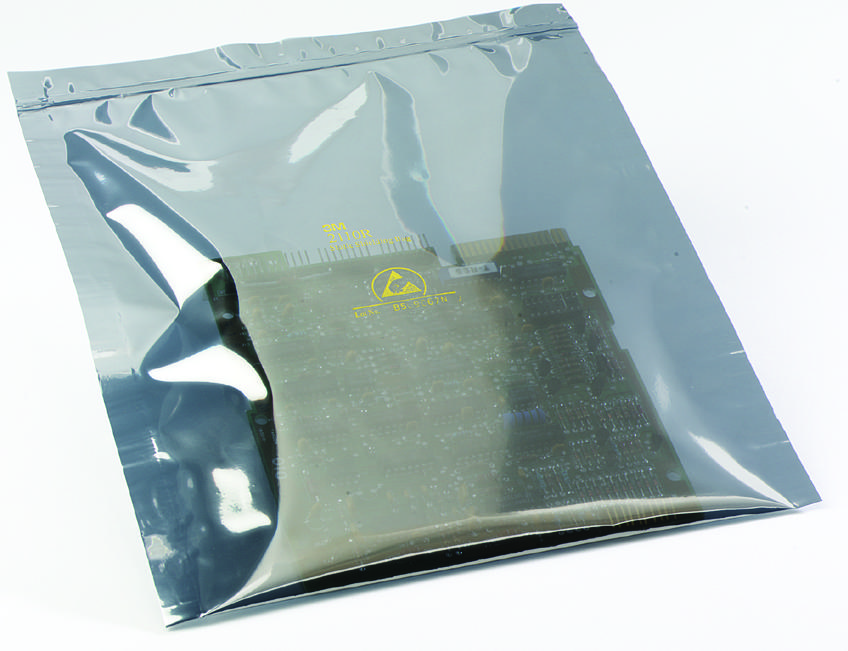
\includegraphics[width=200px]{images/Antistatic-Bag.jpg}
                    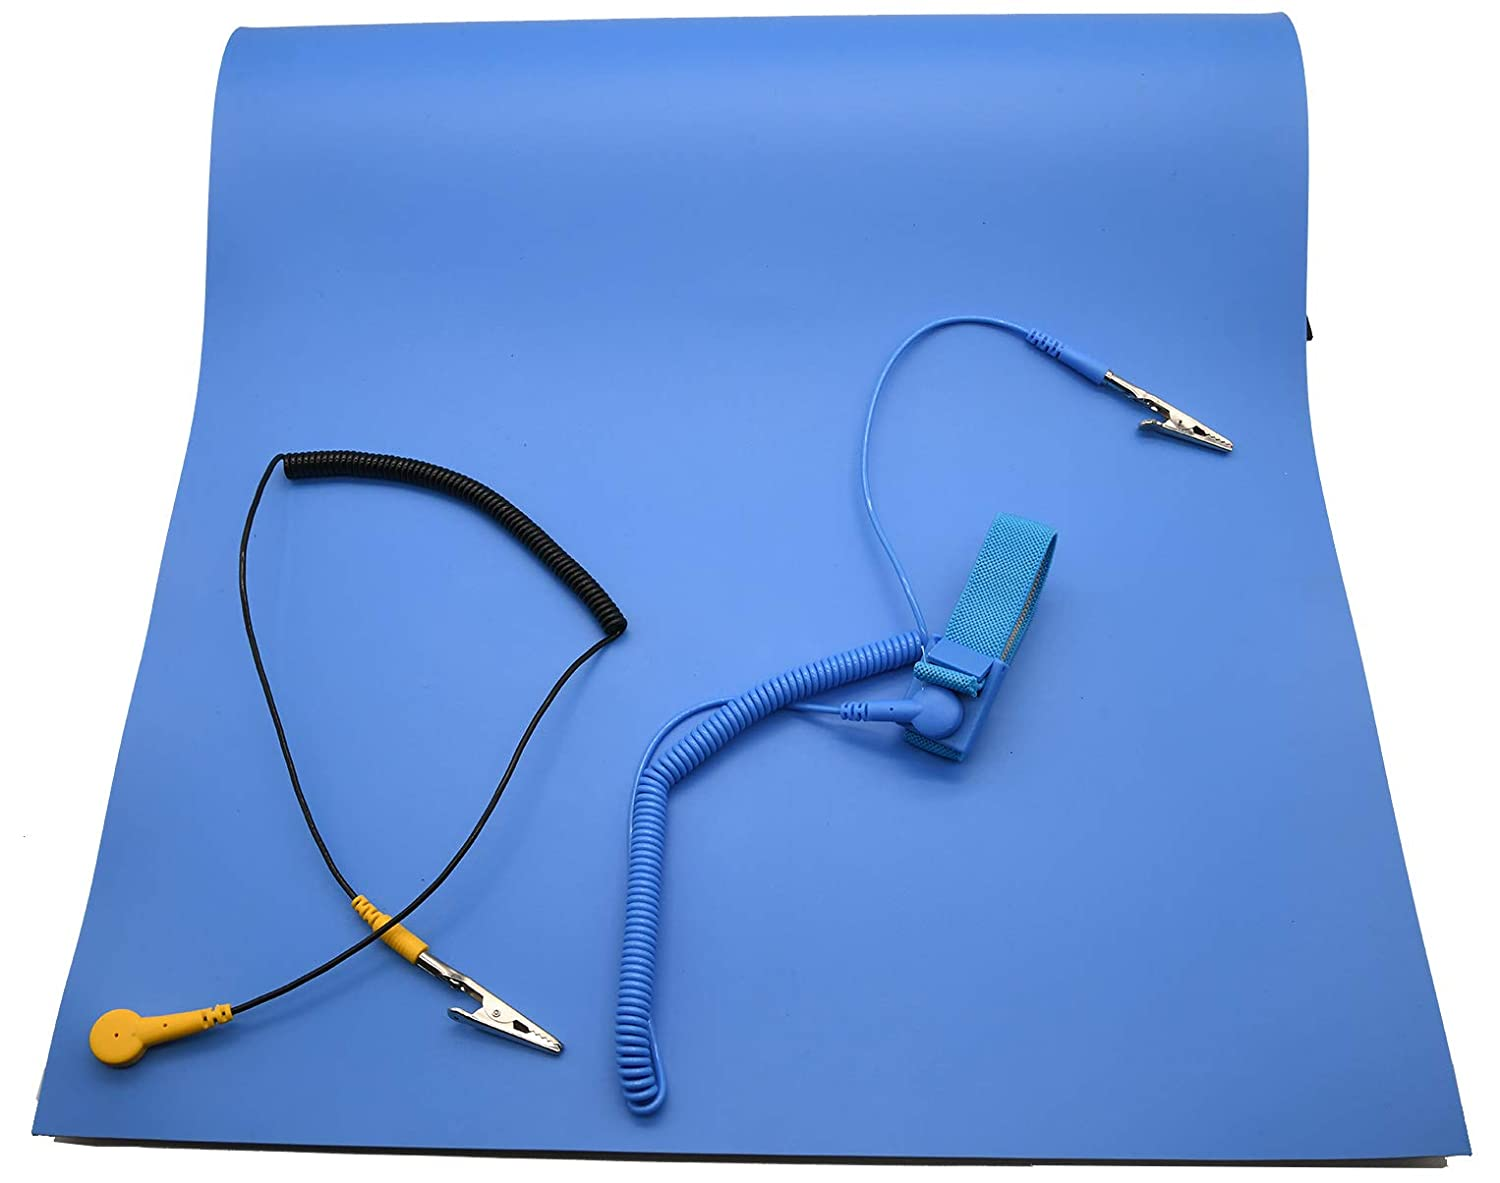
\includegraphics[width=200px]{images/ESD-Mat.jpg}
                \end{center}
    \end{itemize}

    \subsection*{CompTIA Troubleshooting Theory}
    \begin{itemize}
        \item \textbf{CompTIA troubleshooting theory} is a \textbf{set of steps} that \textbf{technicians} can go through to \textbf{troubleshoot problems}.
        \begin{itemize}
            \item There are different approaches to troubleshooting, this is the way that CompTIA prefers.
            \item Specific organizations may also have extra steps they want you to perform (eg paperwork).
        \end{itemize}
        \item \textbf{Always consider policies, procedures, and impacts before implementing changes}.
        \item Troubleshooting steps:
        \begin{enumerate}
            \item \textbf{Identify the problem} | Talk to the user, and discover what issues they are having.
            \item \textbf{Establish a theory of probable cause} | Take a look at the device and identify what may be causing the issue.
            \item \textbf{Test the theory to determine the cause} | Test the theory to see if it is actually the cause, if it is not, go back to step 2. If you are not able to determine the issue, you can always escalate the problem (ask for help).
            \item \textbf{Establish a plan of action to resolve the problem and implement the solution} | Try to resolve the problem.
            \item \textbf{Verify full system functionality and implement preventative measures if applicable} | Ensure the user is satisfied with the solution and implement preventative measures (this could be telling the user how to prevent the issue, or documenting the issue, or escalating the issues, etc).
            \item \textbf{Document findings, actions, and outcomes} | This can be organization specific, but document everything that is required.
        \end{enumerate}
    \end{itemize}

\end{document}